\newpage
\subsection{Caso d'uso UC7 - Visualizzazione API}
\label{UC7}
\begin{figure}[ht]
	\centering
	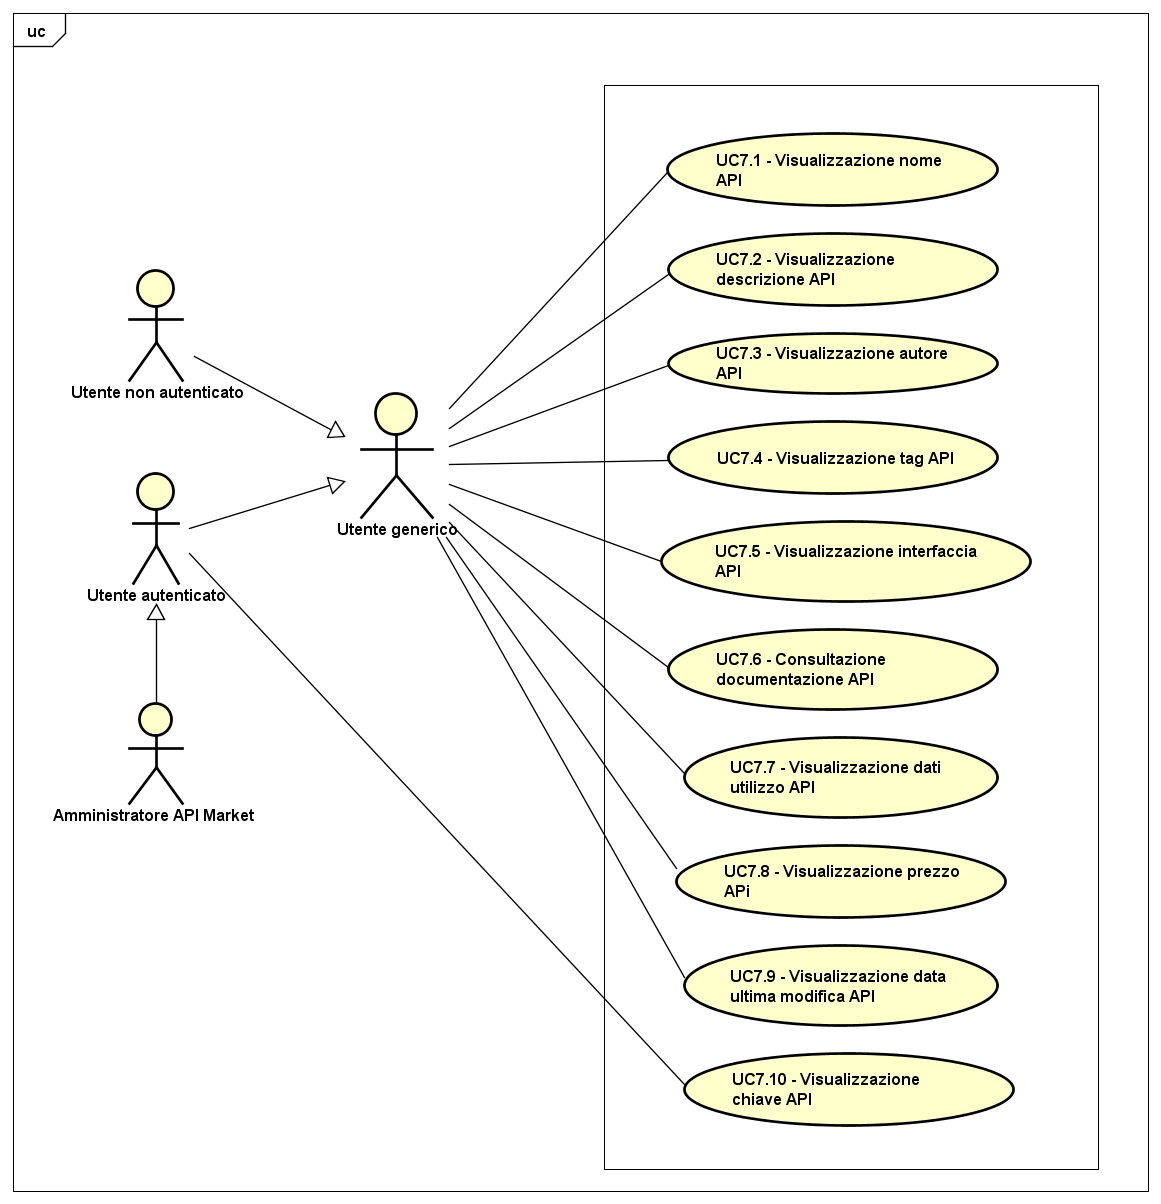
\includegraphics[scale=0.45]{UML/UC7.png}
	\caption{UC7: Visualizzazione API}
\end{figure}

\begin{longtable}{ l | p{11cm}}
	\hline
	\rowcolor{Gray}
	\multicolumn{2}{c}{UC7 - Visualizzazione API}\\
	\hline
	
	 \textbf{Attori} & Utente non autenticato, Utente autenticato, Amministratore API Market \\
	\textbf{Descrizione} & L'attore può visualizzare i dati relativi a un API che ha selezionato tramite la homepage o i risultati di una ricerca  \\
	\textbf{Pre-Condizioni} & L'attore ha selezionato un prodotto per la consultazione \\
	\textbf{Post-Condizioni} & L'attore visualizza la pagina relativa all'API selezionata\\
	\textbf{Scenario Principale} & 
	\begin{enumerate*}[label=(\arabic*.),itemjoin={\newline}]
		\item L'attore visualizza il nome dell'API (UC7.1)
		\item L'attore visualizza la descrizione dell'API (UC7.2)
		\item L'attore visualizza l'autore dell'API (UC7.3)
		\item L'attore può visualizzare l'interfaccia dell'API (UC7.4)
		\item L'attore può consultare la documentazione fornita dall'utente (UC7.5)
		\item L'attore può visualizzare i dati di utilizzo dell'API  (UC7.6)
	\end{enumerate*}\\
\end{longtable}
